\section{Local disk model}\label{setup}
We study the local stability of an inviscid, self-gravitating and
magnetized fluid disk orbiting a central star with
potential $\Phi_*(r,z)$, where $(r,\varphi,z)$ are cylindrical
co-ordinates from the star. We use the shearing box approximation     
\citep{goldreich65b} to consider a small patch of the disk at
a fiducial radius $r=r_0$. The local frame rotates at angular velocity 
$\Omega_0=\Omega(r_0,0)$ about the star, where $r\Omega^2 =
\p\Phi_*/\p r$. We also define $S\equiv-r\p\Omega/\p r$ as the local shear
rate and $\Omega_z^2\equiv\p^2\Phi_*/\p z^2$ as the square of the
local vertical frequency. 

A Cartesian co-ordinate system $(x,y,z)$ is set
up in this local frame, corresponding to the radial, azimuthal and vertical
directions of the global disk, respectively. The shearing box fluid
equations read 
\begin{align} 
  &\frac{\p\rho}{\p t}+\nabla\cdot(\rho\bm{v}) = 0,\\
  &\frac{\p \bm{v}}{\p t} + \bm{v}\cdot\nabla\bm{v} +
  2\Omega_0\hat{\bm{z}}\times\bm{v} = - \frac{1}{\rho}\nabla\Pi +
  \frac{1}{\rho\mu_0}\bm{B}\cdot\nabla\bm{B}
  -\nabla\Phi,\\
  &\frac{\p\bm{B}}{\p t}= \nabla\times\left(\bm{v}\times\bm{B} -
  \eta\nabla\times\bm{B}\right), 
\end{align}
where $\rho$ is the density field; $\bm{v}$ is the total velocity in
the local frame; $\bm{B}$ is the magnetic field which satisfies
$\nabla\cdot~\bm{B}=0$; $\Pi \equiv P +
|\bm{B}|^2/2\mu_0$ is the total pressure, and $\mu_0$ is the vacuum
permeability. We choose a barotropic equation of state, specified
below, so that the gas pressure is given by $P=P(\rho)$. The
resistivity $\eta$ is either uniform or a prescribed function of
height. 


The total potential is $\Phi = \Phi_\mathrm{ext} + \Phi_d$, where
\begin{align}
  \Phi_\mathrm{ext}(x,z) = -\Omega_0 S_0 x^2 +
  \frac{1}{2}\Omega_{z0}^2z^2 
\end{align}
is the effective external potential (central plus centrifugal) in the
shearing box approximation, where $S_0\equiv ~S(r_0,0)$ and
$\Omega_{z0}\equiv\Omega_z(r_0,0)$; 
and the gas potential $\Phi_d$ satisfies Poisson's equation
\begin{align}
  \nabla^2\Phi_d = 4\pi G \rho, 
\end{align}
where $G$ is the gravitational constant. For clarity, hereafter we
drop the subscript $0$ on the frequencies. 



\subsection{Equilibrium disk} 
The unperturbed disk is steady and described by
$\rho=~\rho(z)$, $\bm{B} = B_z\hat{\bm{z}} + B_y\hat{\bm{y}}$ where
$B_{y,z}$ are constants and the toroidal field strength is
$B_y=\epsilon B_z$. The equilibrium 
velocity field is $\bm{v} = -Sx\hat{\bm{y}}$. We consider Keplerian
disks so that $S = 3\Omega/2$ and the epicycle frequency 
$\kappa\equiv\sqrt{2\Omega(2\Omega-S)}=\Omega=\Omega_z$.  
We assume a thin disk and neglect the radial component of the
self-gravitational force in the unperturbed disk.    

The equilibrium density field is obtained by solving
\begin{align}
  &0=\frac{1}{\rho}\frac{d P}{dz} + \Omega_z^2z + \frac{d\Phi_d}{dz},\label{eqm_eqns1}\\
  &\frac{d^2\Phi_d}{dz^2} = 4\pi G \rho.\label{eqm_eqns2}
\end{align}
We consider \begin{inparaenum}[(i)]
\item isothermal disks with $P=c_{s0}^2\rho$\label{iso_eos}; 
\item polytropic disks with $P=K\rho^2$ with $K=c_{s0}^2/2\rho_0$;
\end{inparaenum}
where $\rho_0\equiv\rho(0)$ is the midplane density.
The sound speed $c_s\equiv\sqrt{dP/d\rho}$ 
so that $c_{s0}$ is the global sound speed in the isothermal disk, and
is the midplane sound speed in the polytropic disk. For the polytropic
disk the disk thickness $H$ is such that $\rho(H)=0$. Since the
isothermal disk has no surface, we define $H$ such that
$\rho(H)=10^{-2}\rho_0$. A non-dimensional
measure of the disk thickness is given by 
\begin{align}
  f^{-1} = \frac{H\Omega}{\csmid}, 
\end{align}
and $f$ will appear in subsequent discussions. 


We solve for $\hat{\rho}\equiv\rho/\rho_0$ with 
boundary conditions $\hat{\rho}=1$ and $d\hat{\rho}/dz=0$  at $z=0$. This
is done numerically for isothermal disks and analytically for the
polytropic disk (see Appendix \ref{appen1}). Examples of density
profiles are shown in Fig. \ref{eqm_den}. The normalized density field
is weakly dependent on the strength of self-gravity provided the
$z$-axis is appropriately scaled. 


\begin{figure}
  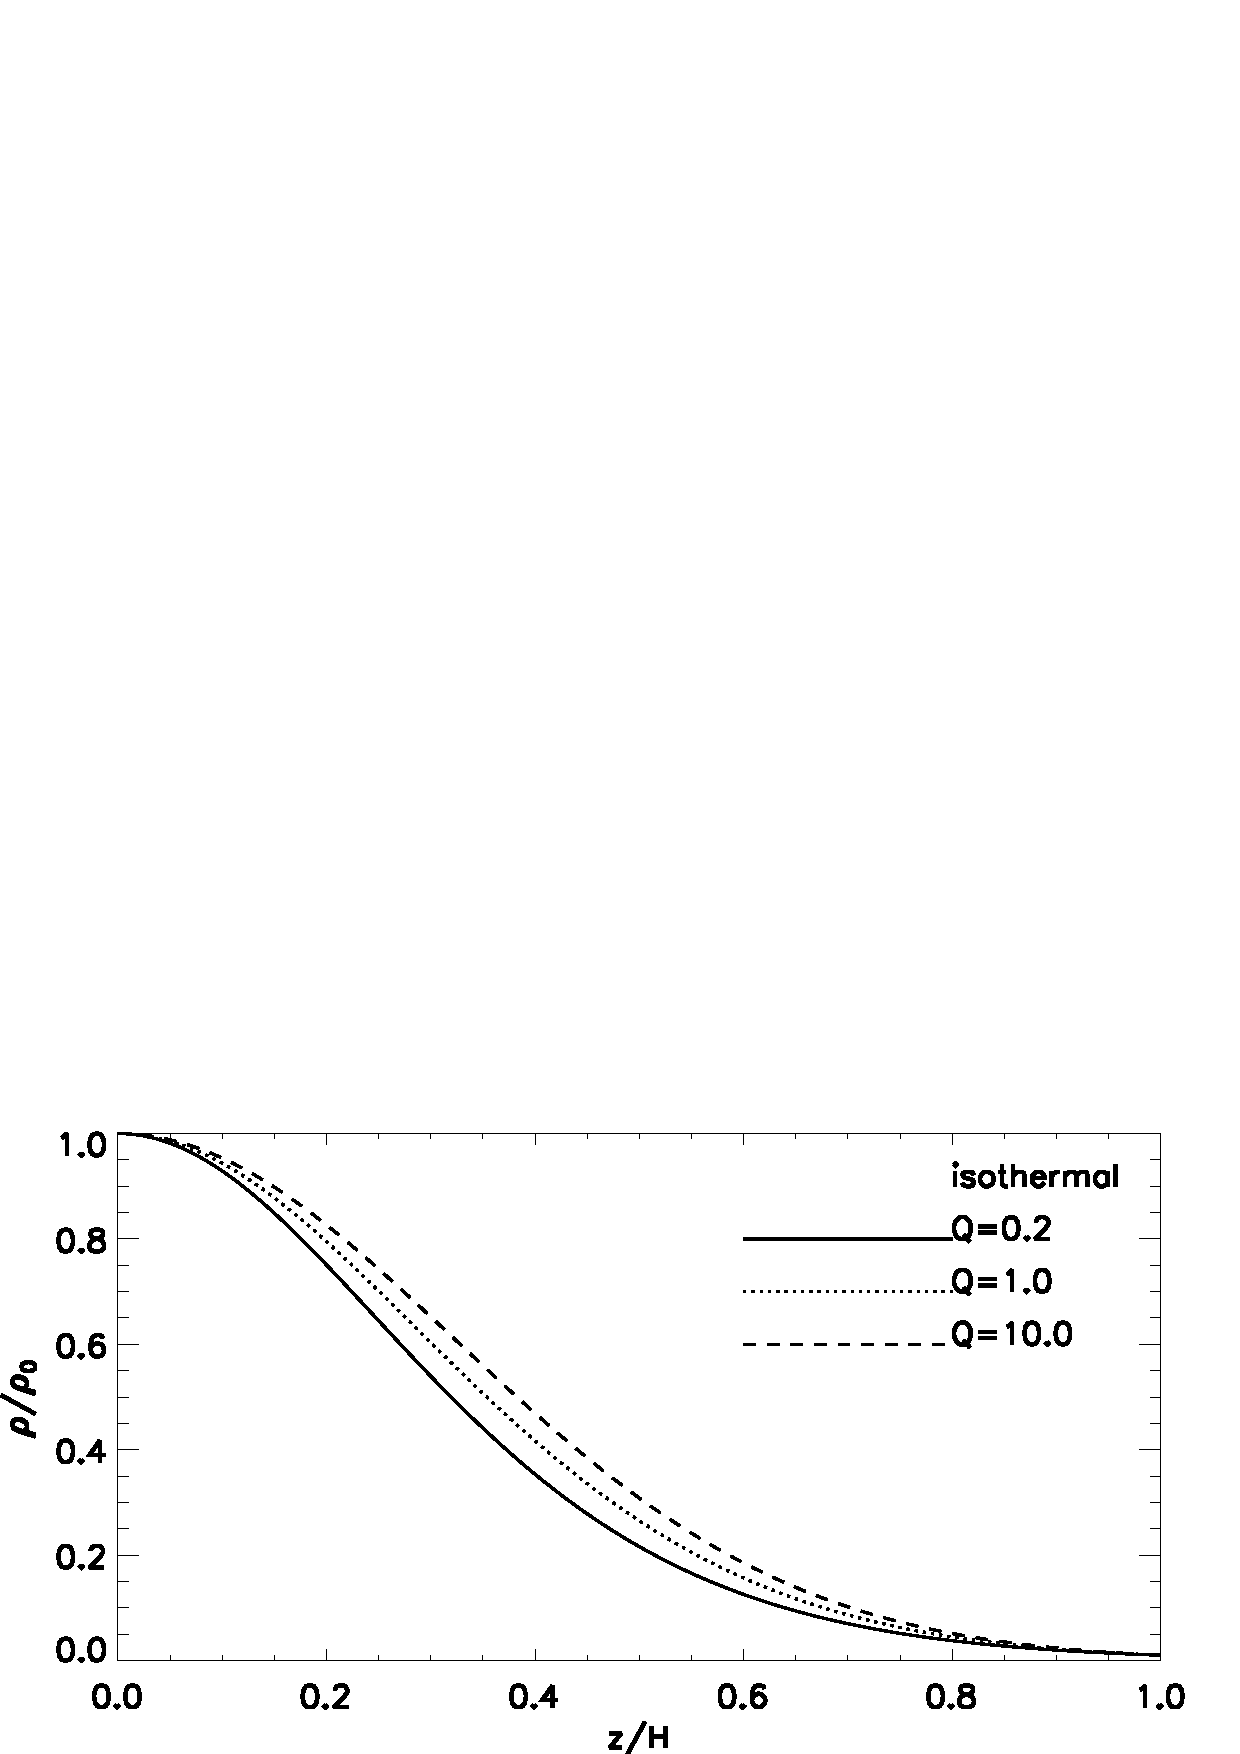
\includegraphics[width=\linewidth,clip=true,trim=0cm 1.5cm 0cm
    0cm]{figures/compare_iso_density} 
  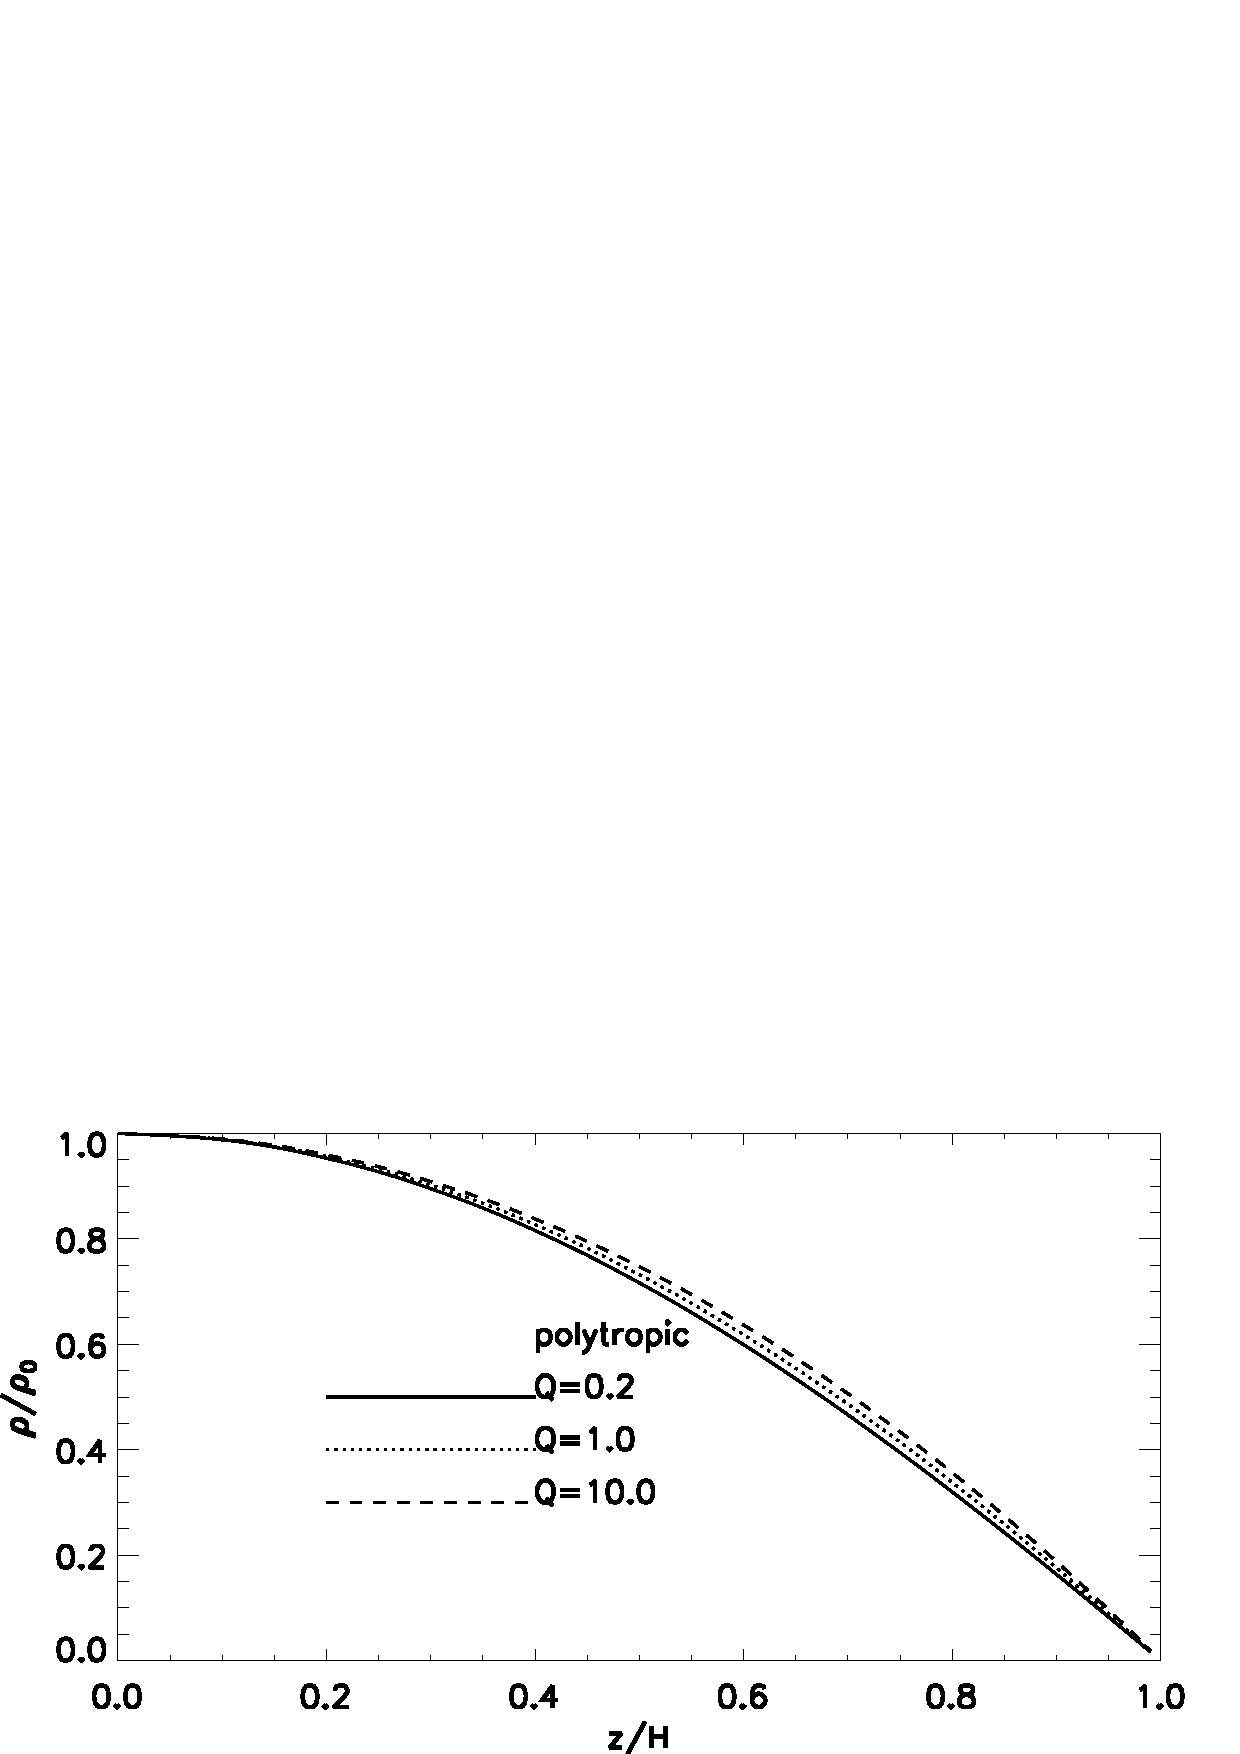
\includegraphics[width=\linewidth,clip=true,trim=0cm 0cm 0cm
    0.9cm]{figures/compare_poly_density} 
  \caption{Equilibrium density field from solving Eq. \ref{eqm_eqns1}
    --- \ref{eqm_eqns2} subject to an isothermal (top) and polytropic
    (bottom) equation of state. Note that the normalization for the
    horizontal axis also depends on the strength of self-gravity,
    i.e. $H=H(Q)$ and is an increasing function of $Q$. 
    \label{eqm_den}}
\end{figure}


\subsection{Resistivity profile}\label{resis_profile}
We adopt constant resistivity or a 
resistivity prescription such that $\eta(z)$ increase towards the
midplane. In the latter case, we follow \cite{fleming03} and use 
the resistivity profile 
\begin{align}
  \eta(z) =
  \sqrt{2}\eta_0\left[\exp{\left(-g_+\right)}+\exp{\left(-g_-\right)}\right]^{-1/2},  
\end{align}
where
\begin{align}
  &g_\pm(z) =  \frac{\Sigma_\pm(z)-\Sigma_0}{\Sigma_*}, \\
  &\Sigma_\pm(z) = \int_{\pm z}^\infty\rho(z^\prime)dz^\prime, \label{sigma_pm}
\end{align}
and $\Sigma_0\equiv\Sigma_{\pm}(0)$, so that $g_\pm(0)=0$ and $\eta_0 
= \eta(0)$. The constant $\Sigma_*$ is chosen such that 
\begin{align}
  \cosh{\left(\frac{\Sigma_0}{\Sigma_*}\right)} =
  \left[\frac{\eta_0}{\eta(\infty)}\right]^2,
\end{align}
and we define $\eta_0/\eta(\infty)\equiv A$ as the conductivity 
boost factor from the midplane to the disk surface. We remark that
once $\rho$ and $d\rho/dz$ are obtained from
Eq. \ref{eqm_eqns1} --- \ref{eqm_eqns2}, the integration for
Eq. \ref{sigma_pm} can be performed implicitly by using Poisson's 
equation. 

We use the Elsasser number $\Lambda$ a non-dimensional measure of
conductivity,
\begin{align} 
  \Lambda \equiv \frac{v_A^2}{\eta\Omega},
\end{align}
where $v_A \equiv B_z/\sqrt{\mu_0\rho}$ is the vertical Alfven speed. 
Because of the density stratification, the Elsasser number 
increases with height even for constant resistivity. The disk may be
considered ideal where $\Lambda \gtrsim 1$. 


\subsection{Disk parameters}
%The main parameters describing the resistive, self-gravitating
%shearing box is as follows. 
The strength of self-gravity is
parametrized by 
\begin{align}
  Q \equiv \frac{\Omega^2}{4\pi G\rho_0}
\end{align}
\citep{mamat10}, which is used to set the midplane density $\rho_0$. 
A relation between $Q$ and the Toomre parameter for gravitational
instability of razor-thin disks, $Q_\mathrm{2D}$, is described in
Appendix \ref{q3d2d}.  

The plasma $\beta$ measures the inverse strength of the  
magnetic field 
\begin{align}
  \beta \equiv \frac{\csmid^2}{v_{A0}^2} =
  \frac{\csmid^2\mu_0\rho_0}{B_z^2},  
\end{align}
where $v_{A0}$ is the midplane Alfven speed. Note that we use 
the vertical field for this definition throughout this paper. 

The strength of conductivity is measured by the midplane Elsasser
number   
\begin{align}
  \Lambda_0 \equiv\Lambda(0) =  \frac{v_{A0}^2}{\eta_0\Omega}. 
\end{align}
For non-uniform resistivity we also specify $A > 1$. 
